\section{Data Encryption Standard (DES)}

\textit{Data Encryption Standard} (DES) adalah cipher blok pertama yang diadopsi
sebagai standar nasional oleh sebuah pemerintahan, dan selama lebih dari dua
dasawarsa ia menjadi tulang punggung kerahasiaan data perbankan, komunikasi
militer, dan jaringan komputer. Nama \textit{Data Encryption Standard} merujuk
pada dokumen standarnya, yaitu FIPS PUB 46 yang diterbitkan pemerintah Amerika
Serikat, sedangkan algoritma yang mendasarinya disebut \textit{Data Encryption
Algorithm} (DEA). Perbedaan nama itu perlu diingat: DES adalah standarnya, DEA
adalah algoritmanya.

Sesuai janji yang dibuat pada Bab~\ref{chap:block-cipher}, DES dibahas lengkap
sampai ke tingkat bit. Seluruh operasinya --- permutasi awal, ekspansi,
substitusi lewat delapan S-box, permutasi $P$, sampai pembangkitan subkunci ---
dinyatakan sebagai tabel posisi bit, bukan sebagai rumus aljabar. Semua tabel itu
disalin apa adanya dari standar, sehingga pembaca dapat mengerjakan DES dengan
kertas dan pensil dan memperoleh hasil yang persis sama dengan hasil program.

\subsection{Sejarah DES}
\label{sec:des-sejarah}

Pada tahun 1972, badan standar Amerika Serikat ketika itu, \textit{National
Bureau of Standards} (NBS; sejak 1988 berganti nama menjadi \textit{National
Institute of Standards and Technology}, NIST), menyadari bahwa lalu lintas data
pemerintah yang tersimpan dan terkirim semakin banyak, sementara tidak ada satu
pun algoritma enkripsi yang dapat dipakai bersama lintas instansi. Setiap
instansi memakai algoritmanya sendiri, sehingga data dari satu instansi tidak
dapat dibaca oleh instansi lain, dan tidak ada yang dapat menilai keamanan
algoritma buatan sendiri. NBS lalu mengumumkan sayembara terbuka untuk merancang
algoritma enkripsi standar.

Kandidat yang akhirnya dipilih berasal dari IBM. Tim riset IBM dipimpin Horst
Feistel, dan cipher rancangan mereka bernama \textbf{Lucifer}. Lucifer sudah
memakai gagasan yang kelak menjadi ciri DES: jaringan berulang yang sekarang
dikenal sebagai \textbf{jaringan Feistel}, dengan blok 128 bit dan kunci
efektif 128 bit. Angka-angka itu jauh lebih besar daripada DES yang kita kenal
sekarang, dan itulah pangkal persoalannya.

Ketika rancangan IBM diserahkan kepada NBS, badan keamanan nasional Amerika
Serikat (NSA) ikut memeriksanya. Hasilnya adalah beberapa perubahan yang
diumumkan pada 1975 dan dibakukan pada 1976 melalui \textit{Federal Register}:

\begin{itemize}
    \item ukuran blok diturunkan dari 128 bit menjadi \textbf{64 bit};
    \item panjang kunci diturunkan dari 128 bit menjadi \textbf{64 bit}, dan
    delapan di antaranya dipakai sebagai bit paritas sehingga kunci efektifnya
    hanya \textbf{56 bit};
    \item delapan S-box diganti dengan rancangan baru yang kriteria
    perancangannya tidak diumumkan.
\end{itemize}

Pemangkasan kunci dari 128 bit menjadi 56 bit mengundang kritik keras. Beberapa
peneliti, terutama Whitfield Diffie dan Martin Hellman, berpendapat bahwa 56 bit
sengaja dipilih agar cukup kecil bagi NSA untuk dipecahkan secara menyeluruh,
sehingga tidak ada pihak lain yang dapat memakai DES tanpa dapat dibaca NSA.
Pemerintah Amerika Serikat bertahan bahwa 56 bit sudah memadai untuk kebutuhan
komersial pada masa itu. Perdebatan itu baru benar-benar selesai dua dasawarsa
kemudian, ketika mesin khusus berhasil memecahkan DES dalam hitungan hari
--- sebagaimana dibahas pada Bagian~\ref{sec:keamanan-des}.

Kecurigaan kedua menyangkut S-box. Mengapa kriterianya dirahasiakan? Jawabannya
baru terbuka pada 1994, ketika Don Coppersmith dari IBM mengungkap bahwa S-box
DES telah dirancang secara sadar untuk tahan terhadap \textbf{kriptanalisis
diferensial}, teknik yang baru ditemukan publik pada 1990 oleh Eli Biham dan Adi
Shamir. Kriteria perancangan S-box dirahasiakan bukan karena kelemahan tersembunyi,
melainkan karena mengungkapkannya sama dengan mengungkap teknik kriptanalisis
yang saat itu masih dikuasai badan keamanan. Peristiwa itu menjadi contoh klasik
bahwa kerahasiaan perancangan dapat menimbulkan ketidakpercayaan meskipun
perancangannya sebenarnya kuat.

Standar DES sendiri hidup panjang. Setelah terbit sebagai FIPS PUB 46 pada
Januari 1977, ia ditegaskan kembali pada 1983 dan 1988 (FIPS 46-1), diperbarui
pada 1993 (FIPS 46-2), dan pada 1999 (FIPS 46-3) diperluas dengan Triple DES.
Standar itu baru resmi ditarik pada 2005, setelah Advanced Encryption Standard
menggantikannya.

\subsection{Karakteristik Teknis DES}

Parameter DES yang perlu dihafal sebelum masuk ke mekanismenya adalah:

\begin{itemize}
    \item \textbf{Ukuran blok}: 64 bit, baik untuk plainteks maupun cipherteks.
    \item \textbf{Ukuran kunci}: kunci eksternal 64 bit, tetapi bit pada posisi
    8, 16, 24, 32, 40, 48, 56, dan 64 adalah bit paritas ganjil dan
    \textbf{diabaikan} oleh algoritma. Kunci efektifnya karena itu hanya
    \textbf{56 bit}.
    \item \textbf{Struktur}: jaringan Feistel dengan \textbf{16 putaran}.
    \item \textbf{Subkunci}: 16 buah kunci putaran, masing-masing 48 bit, yang
    diturunkan dari kunci efektif 56 bit.
    \item \textbf{Jumlah putaran minimum}: DES memakai 16 putaran; seperti
    dibahas pada Bagian~\ref{sec:keamanan-des}, DES dengan kurang dari 16 putaran
    dapat ditembus secara sistematis.
\end{itemize}

Bit paritas pada kunci bukan bagian dari keamanan; fungsinya historis, yaitu
memungkinkan deteksi kesalahan pengetikan kunci ketika kunci masih dibagikan
dalam bentuk deretan angka. Karena paritasnya ganjil, setiap byte kunci selalu
memuat jumlah bit $1$ yang ganjil. Perlu ditegaskan bahwa paritas ini tidak
menambah sedikit pun kekuatan kunci: penyerang tetap hanya perlu menebak 56 bit,
bukan 64 bit.

\subsection{Mekanisme Kerja DES}

Enkripsi DES berlangsung dalam tiga tahap:

\begin{enumerate}
    \item \textbf{Permutasi awal} (\textit{Initial Permutation}, IP) mengacak
    urutan 64 bit plainteks.
    \item \textbf{Enam belas putaran Feistel} (disebut tahap
    \textit{enciphering}) mengolah hasil permutasi awal dengan 16 subkunci
    $K_1, K_2, \dots, K_{16}$.
    \item \textbf{Inversi permutasi awal} ($\text{IP}^{-1}$) mengembalikan bit
    ke urutan akhir untuk membentuk cipherteks.
\end{enumerate}

Skema menyeluruhnya tampak pada Gambar~\ref{fig:skema-enkripsi-des}. Perhatikan
satu hal yang sering menimbulkan kebingungan: permutasi awal dan inversinya
sebenarnya \textbf{tidak menambah keamanan sama sekali}, karena keduanya tidak
bergantung pada kunci dan bersifat tetap. Keduanya hanya bagian dari rancangan
perangkat keras awal DES. Yang benar-benar mengandung kunci adalah 16 putaran
Feistel di antaranya.

Dekripsi DES dilakukan dengan algoritma yang sama persis. Karena struktur
Feistel bersifat reversibel dengan sendirinya (Bab~\ref{chap:block-cipher}),
dekripsi hanya perlu menjalankan 16 putaran yang sama dengan urutan subkunci
dibalik, yaitu $K_{16}$ turun sampai $K_1$. Tidak ada fungsi inversi S-box yang
perlu dibuat. Sifat inilah yang membuat DES hemat perangkat keras dan menjadi
alasan struktural mengapa DES memakai jaringan Feistel, bukan jaringan SPN
seperti AES.

\subsection{Permutasi Awal dan Inversinya}

Permutasi awal IP dinyatakan sebagai tabel 64 bilangan. Angka pada posisi ke-$i$
tabel menyatakan bahwa bit keluaran ke-$i$ diambil dari bit masukan nomor itu.
Membaca tabel secara baris demi baris, bit pertama keluaran adalah bit masukan
58, bit kedua adalah bit masukan 50, dan seterusnya. Tabel~\ref{tab:ip-des}
menyajikan IP bersama inversinya, $\text{IP}^{-1}$; keduanya disusun sebagai
delapan baris yang masing-masing memuat delapan bilangan.

\begin{table}[htbp]
\centering
\small
\setlength{\tabcolsep}{4pt}
\begin{tabular}{@{}*{8}{c}@{}}
\multicolumn{8}{c}{\textbf{Permutasi Awal (IP)}} \\
\hline
58 & 50 & 42 & 34 & 26 & 18 & 10 & 2 \\
60 & 52 & 44 & 36 & 28 & 20 & 12 & 4 \\
62 & 54 & 46 & 38 & 30 & 22 & 14 & 6 \\
64 & 56 & 48 & 40 & 32 & 24 & 16 & 8 \\
57 & 49 & 41 & 33 & 25 & 17 & 9 & 1 \\
59 & 51 & 43 & 35 & 27 & 19 & 11 & 3 \\
61 & 53 & 45 & 37 & 29 & 21 & 13 & 5 \\
63 & 55 & 47 & 39 & 31 & 23 & 15 & 7 \\
\end{tabular}
\hspace{1.2em}
\begin{tabular}{@{}*{8}{c}@{}}
\multicolumn{8}{c}{\textbf{Invers Permutasi Awal ($\text{IP}^{-1}$)}} \\
\hline
40 & 8 & 48 & 16 & 56 & 24 & 64 & 32 \\
39 & 7 & 47 & 15 & 55 & 23 & 63 & 31 \\
38 & 6 & 46 & 14 & 54 & 22 & 62 & 30 \\
37 & 5 & 45 & 13 & 53 & 21 & 61 & 29 \\
36 & 4 & 44 & 12 & 52 & 20 & 60 & 28 \\
35 & 3 & 43 & 11 & 51 & 19 & 59 & 27 \\
34 & 2 & 42 & 10 & 50 & 18 & 58 & 26 \\
33 & 1 & 41 & 9 & 49 & 17 & 57 & 25 \\
\end{tabular}
\caption{Tabel bit permutasi awal DES dan inversinya}
\label{tab:ip-des}
\sumber{Data dari FIPS PUB 46-3; disusun ulang dari Munir, \textit{IF4020 Kriptografi}, ITB.}
\end{table}

Perlu dipahami bahwa IP dan $\text{IP}^{-1}$ bukan pengacakan acak. Bit masukan
yang semula berdekatan justru sering tetap berdekatan, tetapi berpindah dari
separuh kiri ke separuh kanan. Sebagai contoh, delapan bit pertama keluaran IP
diambil dari bit masukan $58, 50, 42, 34, 26, 18, 10, 2$, yaitu bit-bit dari
separuh kanan blok, sedangkan delapan bit berikutnya diambil dari
$60, 52, 44, 36, 28, 20, 12, 4$. Pola semacam ini bukan kebetulan: perancang IP
bermaksud mencampur separuh kiri dan separuh kanan blok sebelum putaran pertama,
sehingga tidak ada separuh yang masuk ke jaringan Feistel tanpa pernah
bercampur. Namun sekali lagi, karena IP tidak bergantung pada kunci,
penyerang dapat menghitungnya sendiri tanpa biaya. Keamanan DES seluruhnya
bersandar pada 16 putaran Feistel dan pembangkitan subkuncinya.

\subsection{Struktur Putaran dan Fungsi \texorpdfstring{$f$}{f}}

Seperti semua cipher jaringan Feistel (Bab~\ref{chap:block-cipher}), hasil IP
dipecah menjadi dua separuh 32 bit, $L_0$ dan $R_0$, dan setiap putaran
berlangsung menurut
\begin{equation}
L_i = R_{i-1}, \qquad R_i = L_{i-1} \oplus f(R_{i-1}, K_i),
\label{eq:des-putaran}
\end{equation}
untuk $i = 1, 2, \dots, 16$. Setelah putaran ke-16, kedua separuh \textbf{tidak}
ditukar lagi; blok hasil putaran terakhir langsung disusun sebagai
$R_{16} \parallel L_{16}$ dan masuk ke $\text{IP}^{-1}$. Pembalikan urutan ini
adalah kekhususan jaringan Feistel yang membuat dekripsi dapat memakai mesin yang
sama.

Inti DES ada pada fungsi $f$, yang menerima blok 32 bit dan subkunci 48 bit, lalu
menghasilkan 32 bit. Fungsi itu bekerja dalam empat langkah (fungsi-f-des.png
pada Gambar~\ref{fig:fungsi-f-des}):

\begin{enumerate}
    \item \textbf{Ekspansi $E$} mengubah blok 32 bit menjadi 48 bit dengan
    menyalin ulang 16 bit tertentu sehingga delapan bit masukan muncul di dua
    posisi keluaran sekaligus.
    \item \textbf{XOR} hasil ekspansi dengan subkunci $K_i$ yang juga 48 bit.
    \item \textbf{Substitusi S-box}: 48 bit hasil XOR dipecah menjadi delapan
    kelompok enam bit, dan tiap kelompok disubstitusi oleh S-box $S_1$ sampai
    $S_8$ menjadi empat bit, sehingga 48 bit kembali menjadi 32 bit.
    \item \textbf{Permutasi $P$} mengacak urutan 32 bit hasil S-box.
\end{enumerate}

Secara ringkas,
\begin{equation}
f(R, K) = P\bigl( S_1(B_1) \parallel S_2(B_2) \parallel \dots \parallel S_8(B_8) \bigr),
\label{eq:des-f}
\end{equation}
dengan $B_j$ adalah kelompok 6 bit ke-$j$ dari $E(R) \oplus K$.

Tabel ekspansi $E$ dan permutasi $P$ disajikan pada Tabel~\ref{tab:ep-des}.
Ekspansi $E$ sengaja dibuat tumpang tindih: bit ke-4 masukan muncul di kelompok
pertama dan kelompok kedua, bit ke-5 muncul di kelompok kedua dan ketiga, dan
seterusnya. Akibat tumpang tindih itu, satu bit blok kanan mempengaruhi dua
kelompok S-box yang berbeda, sehingga pengaruhnya menyebar lebih cepat.
Permutasi $P$ melengkapi penyebaran itu dengan memindahkan bit-bit hasil S-box ke
posisi yang berjauhan, misalnya bit keluaran pertama dan ketiga S-box $S_1$
dipindahkan ke posisi 16 dan 20.

\begin{table}[htbp]
\centering
\small
\setlength{\tabcolsep}{4pt}
\begin{tabular}{@{}*{6}{c}@{}}
\multicolumn{6}{c}{\textbf{Fungsi Ekspansi ($E$)}} \\
\hline
32 & 1 & 2 & 3 & 4 & 5 \\
4 & 5 & 6 & 7 & 8 & 9 \\
8 & 9 & 10 & 11 & 12 & 13 \\
12 & 13 & 14 & 15 & 16 & 17 \\
16 & 17 & 18 & 19 & 20 & 21 \\
20 & 21 & 22 & 23 & 24 & 25 \\
24 & 25 & 26 & 27 & 28 & 29 \\
28 & 29 & 30 & 31 & 32 & 1 \\
\end{tabular}
\hspace{1.5em}
\begin{tabular}{@{}*{4}{c}@{}}
\multicolumn{4}{c}{\textbf{Permutasi $P$}} \\
\hline
16 & 7 & 20 & 21 \\
29 & 12 & 28 & 17 \\
1 & 15 & 23 & 26 \\
5 & 18 & 31 & 10 \\
2 & 8 & 24 & 14 \\
32 & 27 & 3 & 9 \\
19 & 13 & 30 & 6 \\
22 & 11 & 4 & 25 \\
\end{tabular}
\caption{Tabel bit ekspansi $E$ (32 bit menjadi 48 bit) dan permutasi $P$ pada fungsi $f$ DES}
\label{tab:ep-des}
\sumber{Data dari FIPS PUB 46-3; disusun ulang dari Munir, \textit{IF4020 Kriptografi}, ITB.}
\end{table}

\begin{figure}[htbp]
    \centering
    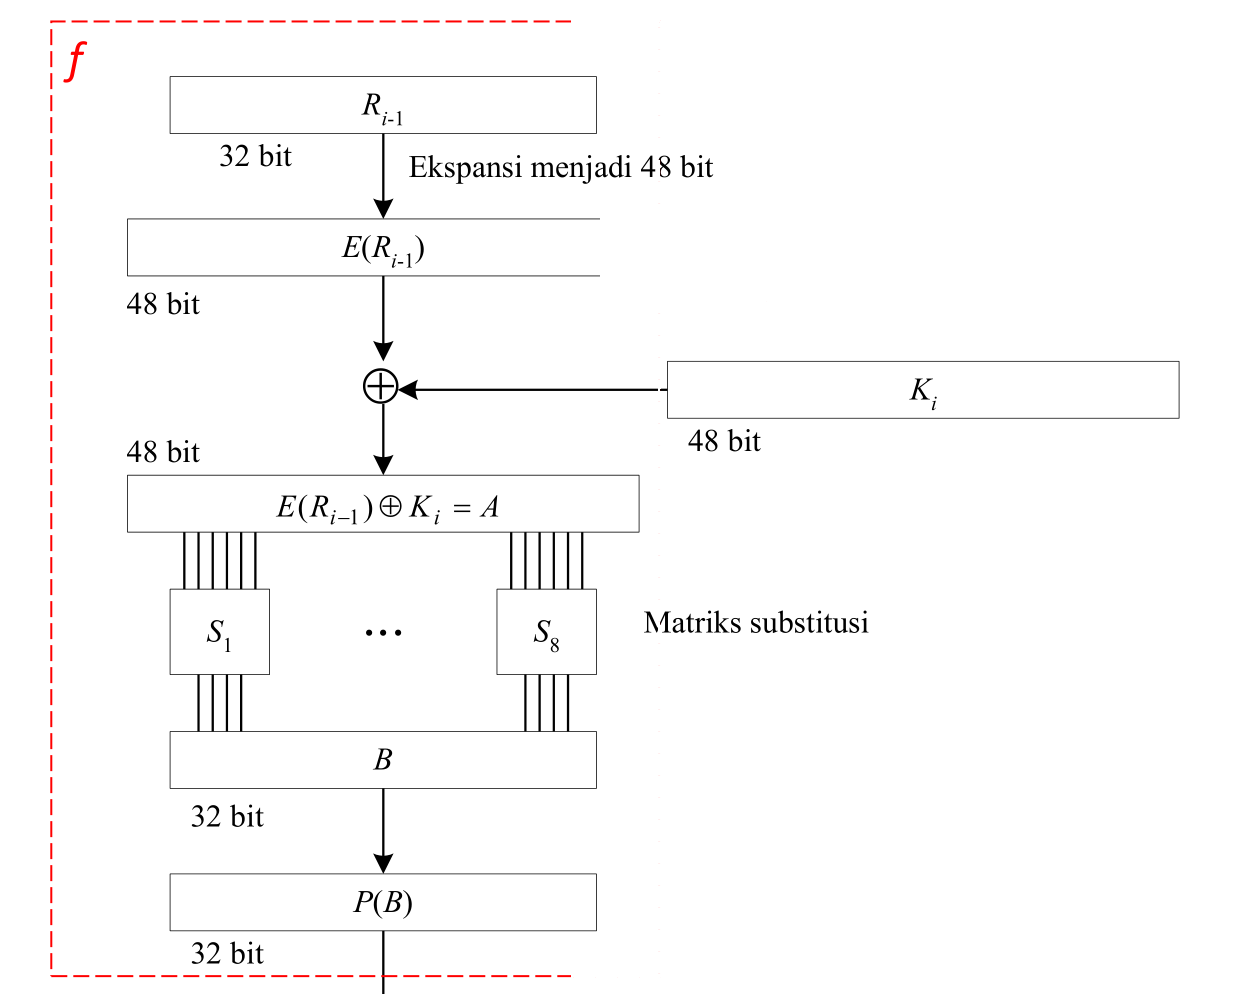
\includegraphics[width=0.9\linewidth, height=0.82\textheight, keepaspectratio]{figures/fungsi-f-des.png}
    \caption{Komputasi fungsi $f$ pada DES: ekspansi blok kanan 32 bit menjadi 48 bit, XOR dengan subkunci, substitusi melalui delapan S-box, dan permutasi $P$}
    \label{fig:fungsi-f-des}
    \sumber{Munir, \textit{IF4020 Kriptografi}, ITB.}
\end{figure}

\subsection{Delapan S-box DES}

S-box adalah satu-satunya bagian DES yang nirlanjar, dan karena itu ia memikul
seluruh beban kerahasiaan. Setiap S-box $S_j$ menerima enam bit masukan dan
menghasilkan empat bit keluaran, yang berarti ia adalah pemetaan dari himpunan
64 nilai ke himpunan 16 nilai. Tabelnya disusun sebagai matriks $4 \times 16$:
nomor baris ditentukan oleh bit pertama dan bit keenam masukan (digabung sebagai
bilangan 2 bit), sedangkan nomor kolomnya ditentukan oleh bit kedua sampai bit
kelima (bilangan 4 bit). Jadi masukan $b_1b_2b_3b_4b_5b_6$ dibaca sebagai
$\text{baris} = (b_1b_6)_2$ dan $\text{kolom} = (b_2b_3b_4b_5)_2$.

Kelapan tabelnya disajikan pada Tabel~\ref{tab:sbox-des}. Cara membacanya
diperlihatkan pada Contoh~\ref{ex:des-sbox} di bagian akhir bab, tetapi polanya
dapat langsung dilihat: pada $S_1$, masukan $\code{011000}$ berarti baris
$0$ (dari bit $0$ dan $0$) dan kolom $12$ (dari bit $1100$), sehingga keluarannya
adalah entri baris 0 kolom 12, yaitu $5$ atau $\code{0101}$ dalam biner.

\begin{table}[htbp]
\centering
\footnotesize
\setlength{\tabcolsep}{3.5pt}
\begin{tabular}{@{}l@{\hspace{5pt}}*{16}{c}@{}}
$S_1$ & 14 & 4 & 13 & 1 & 2 & 15 & 11 & 8 & 3 & 10 & 6 & 12 & 5 & 9 & 0 & 7 \\
      & 0 & 15 & 7 & 4 & 14 & 2 & 13 & 1 & 10 & 6 & 12 & 11 & 9 & 5 & 3 & 8 \\
      & 4 & 1 & 14 & 8 & 13 & 6 & 2 & 11 & 15 & 12 & 9 & 7 & 3 & 10 & 5 & 0 \\
      & 15 & 12 & 8 & 2 & 4 & 9 & 1 & 7 & 5 & 11 & 3 & 14 & 10 & 0 & 6 & 13 \\[4pt]
$S_2$ & 15 & 1 & 8 & 14 & 6 & 11 & 3 & 4 & 9 & 7 & 2 & 13 & 12 & 0 & 5 & 10 \\
      & 3 & 13 & 4 & 7 & 15 & 2 & 8 & 14 & 12 & 0 & 1 & 10 & 6 & 9 & 11 & 5 \\
      & 0 & 14 & 7 & 11 & 10 & 4 & 13 & 1 & 5 & 8 & 12 & 6 & 9 & 3 & 2 & 15 \\
      & 13 & 8 & 10 & 1 & 3 & 15 & 4 & 2 & 11 & 6 & 7 & 12 & 0 & 5 & 14 & 9 \\[4pt]
$S_3$ & 10 & 0 & 9 & 14 & 6 & 3 & 15 & 5 & 1 & 13 & 12 & 7 & 11 & 4 & 2 & 8 \\
      & 13 & 7 & 0 & 9 & 3 & 4 & 6 & 10 & 2 & 8 & 5 & 14 & 12 & 11 & 15 & 1 \\
      & 13 & 6 & 4 & 9 & 8 & 15 & 3 & 0 & 11 & 1 & 2 & 12 & 5 & 10 & 14 & 7 \\
      & 1 & 10 & 13 & 0 & 6 & 9 & 8 & 7 & 4 & 15 & 14 & 3 & 11 & 5 & 2 & 12 \\[4pt]
$S_4$ & 7 & 13 & 14 & 3 & 0 & 6 & 9 & 10 & 1 & 2 & 8 & 5 & 11 & 12 & 4 & 15 \\
      & 13 & 8 & 11 & 5 & 6 & 15 & 0 & 3 & 4 & 7 & 2 & 12 & 1 & 10 & 14 & 9 \\
      & 10 & 6 & 9 & 0 & 12 & 11 & 7 & 13 & 15 & 1 & 3 & 14 & 5 & 2 & 8 & 4 \\
      & 3 & 15 & 0 & 6 & 10 & 1 & 13 & 8 & 9 & 4 & 5 & 11 & 12 & 7 & 2 & 14 \\[4pt]
$S_5$ & 2 & 12 & 4 & 1 & 7 & 10 & 11 & 6 & 8 & 5 & 3 & 15 & 13 & 0 & 14 & 9 \\
      & 14 & 11 & 2 & 12 & 4 & 7 & 13 & 1 & 5 & 0 & 15 & 10 & 3 & 9 & 8 & 6 \\
      & 4 & 2 & 1 & 11 & 10 & 13 & 7 & 8 & 15 & 9 & 12 & 5 & 6 & 3 & 0 & 14 \\
      & 11 & 8 & 12 & 7 & 1 & 14 & 2 & 13 & 6 & 15 & 0 & 9 & 10 & 4 & 5 & 3 \\[4pt]
$S_6$ & 12 & 1 & 10 & 15 & 9 & 2 & 6 & 8 & 0 & 13 & 3 & 4 & 14 & 7 & 5 & 11 \\
      & 10 & 15 & 4 & 2 & 7 & 12 & 9 & 5 & 6 & 1 & 13 & 14 & 0 & 11 & 3 & 8 \\
      & 9 & 14 & 15 & 5 & 2 & 8 & 12 & 3 & 7 & 0 & 4 & 10 & 1 & 13 & 11 & 6 \\
      & 4 & 3 & 2 & 12 & 9 & 5 & 15 & 10 & 11 & 14 & 1 & 7 & 6 & 0 & 8 & 13 \\[4pt]
$S_7$ & 4 & 11 & 2 & 14 & 15 & 0 & 8 & 13 & 3 & 12 & 9 & 7 & 5 & 10 & 6 & 1 \\
      & 13 & 0 & 11 & 7 & 4 & 9 & 1 & 10 & 14 & 3 & 5 & 12 & 2 & 15 & 8 & 6 \\
      & 1 & 4 & 11 & 13 & 12 & 3 & 7 & 14 & 10 & 15 & 6 & 8 & 0 & 5 & 9 & 2 \\
      & 6 & 11 & 13 & 8 & 1 & 4 & 10 & 7 & 9 & 5 & 0 & 15 & 14 & 2 & 3 & 12 \\[4pt]
$S_8$ & 13 & 2 & 8 & 4 & 6 & 15 & 11 & 1 & 10 & 9 & 3 & 14 & 5 & 0 & 12 & 7 \\
      & 1 & 15 & 13 & 8 & 10 & 3 & 7 & 4 & 12 & 5 & 6 & 11 & 0 & 14 & 9 & 2 \\
      & 7 & 11 & 4 & 1 & 9 & 12 & 14 & 2 & 0 & 6 & 10 & 13 & 15 & 3 & 5 & 8 \\
      & 2 & 1 & 14 & 7 & 4 & 10 & 8 & 13 & 15 & 12 & 9 & 0 & 3 & 5 & 6 & 11 \\
\end{tabular}
\caption{Delapan S-box DES. Setiap tabel memetakan 6 bit ke 4 bit; baris 0--3, kolom 0--15}
\label{tab:sbox-des}
\sumber{Data dari FIPS PUB 46-3; disusun ulang dari Munir, \textit{IF4020 Kriptografi}, ITB.}
\end{table}

Ada dua sifat S-box yang penting untuk dipahami. Pertama, tidak ada S-box yang
merupakan fungsi linier atau affine atas masukannya; hal itu dapat diperiksa
langsung dari tabelnya, misalnya $\code{000000}$ pada $S_1$ menghasilkan $14$
bukan $0$. Kedua, setiap nilai keluaran 4 bit muncul tepat sekali pada setiap
baris --- sifat itu disebut \textit{permutasi per baris} --- sehingga tidak ada
keluaran yang hilang. Kedua sifat itu beserta sejumlah kriteria lain dipilih
untuk memaksimumkan ketahanan terhadap kriptanalisis diferensial dan linier.

\subsection{Pembangkitan Kunci Putaran}

Kunci eksternal 64 bit harus diubah menjadi 16 subkunci 48 bit. Prosesnya,
yang tampak pada Gambar~\ref{fig:pembangkitan-kunci-des}, berjalan dalam tiga
langkah:

\begin{enumerate}
    \item \textbf{PC-1} (\textit{Permuted Choice 1}) memilih 56 bit dari kunci 64
    bit, yaitu membuang delapan bit paritas. Hasilnya langsung dipecah menjadi
    dua register 28 bit, $C_0$ dan $D_0$.
    \item \textbf{Pergeseran siklik} (\textit{left shift}) dilakukan pada $C_i$ dan
    $D_i$ pada setiap putaran menurut jadwal pada Tabel~\ref{tab:jadwal-geser-des}.
    \item \textbf{PC-2} (\textit{Permuted Choice 2}) memilih 48 dari 56 bit hasil
    gabungan $C_i \parallel D_i$ untuk menjadi subkunci $K_i$.
\end{enumerate}

Perhatikan bahwa \textbf{setiap bit kunci tidak selalu terpakai di setiap
putaran}. PC-2 hanya memilih 48 dari 56 bit yang tersedia, sehingga delapan bit
selalu tersisa dan berganti-ganti dari putaran ke putaran. Jadi tidak benar
bahwa subkunci $K_1, \dots, K_{16}$ bersama-sama memuat seluruh 56 bit kunci di
setiap putaran; yang benar adalah setiap bit kunci muncul pada sebagian besar
putaran, tetapi tidak semua.

Secara formal, dengan $C_0 \parallel D_0 = \mathrm{PC1}(K)$ dan
$\mathrm{LS}_i$ menyatakan pergeseran siklik ke kiri sejauh $s_i$ bit,
\begin{equation}
C_i = \mathrm{LS}_{s_i}(C_{i-1}), \qquad D_i = \mathrm{LS}_{s_i}(D_{i-1}),
\qquad K_i = \mathrm{PC2}(C_i \parallel D_i).
\label{eq:des-subkunci}
\end{equation}
Jadwal pergeseran $s_i$ sengaja tidak seragam. Pada putaran 1, 2, 9, dan 16
pergeserannya satu bit, sedangkan pada putaran lain dua bit.

\begin{table}[htbp]
\centering
\small
\setlength{\tabcolsep}{4pt}
\begin{tabular}{@{}l*{16}{c}@{}}
\hline
\textbf{Putaran $i$} & 1 & 2 & 3 & 4 & 5 & 6 & 7 & 8 & 9 & 10 & 11 & 12 & 13 & 14 & 15 & 16 \\
\hline
\textbf{Pergeseran $s_i$} & 1 & 1 & 2 & 2 & 2 & 2 & 2 & 2 & 1 & 2 & 2 & 2 & 2 & 2 & 2 & 1 \\
\hline
\end{tabular}
\caption{Jadwal pergeseran siklik kiri pada pembangkitan subkunci DES}
\label{tab:jadwal-geser-des}
\sumber{Data dari FIPS PUB 46-3.}
\end{table}

Tabel PC-1 dan PC-2 disajikan pada Tabel~\ref{tab:pc-des}. Pada PC-1, empat baris
pertama membentuk $C_0$ dan empat baris terakhir membentuk $D_0$. Perhatikan
bahwa tidak ada bilangan 8, 16, 24, 32, 40, 48, 56, dan 64 di dalam PC-1;
itulah cara kedelapan bit paritas dibuang. Pada PC-2, susunannya
mencampur bit-bit dari $C$ dan $D$ secara berselang-seling, sehingga setiap
subkunci memuat bit dari kedua separuh kunci.

\begin{table}[htbp]
\centering
\small
\setlength{\tabcolsep}{4pt}
\begin{tabular}{@{}*{7}{c}@{}}
\multicolumn{7}{c}{\textbf{PC-1 (64 bit menjadi 56 bit)}} \\
\hline
57 & 49 & 41 & 33 & 25 & 17 & 9 \\
1 & 58 & 50 & 42 & 34 & 26 & 18 \\
10 & 2 & 59 & 51 & 43 & 35 & 27 \\
19 & 11 & 3 & 60 & 52 & 44 & 36 \\
\hline
63 & 55 & 47 & 39 & 31 & 23 & 15 \\
7 & 62 & 54 & 46 & 38 & 30 & 22 \\
14 & 6 & 61 & 53 & 45 & 37 & 29 \\
21 & 13 & 5 & 28 & 20 & 12 & 4 \\
\end{tabular}
\hspace{2em}
\begin{tabular}{@{}*{6}{c}@{}}
\multicolumn{6}{c}{\textbf{PC-2 (56 bit menjadi 48 bit)}} \\
\hline
14 & 17 & 11 & 24 & 1 & 5 \\
3 & 28 & 15 & 6 & 21 & 10 \\
23 & 19 & 12 & 4 & 26 & 8 \\
16 & 7 & 27 & 20 & 13 & 2 \\
41 & 52 & 31 & 37 & 47 & 55 \\
30 & 40 & 51 & 45 & 33 & 48 \\
44 & 49 & 39 & 56 & 34 & 53 \\
46 & 42 & 50 & 36 & 29 & 32 \\
\end{tabular}
\caption{Tabel bit pembangkitan kunci DES: PC-1 (empat baris atas menjadi $C_0$, empat baris bawah menjadi $D_0$) dan PC-2}
\label{tab:pc-des}
\sumber{Data dari FIPS PUB 46-3; disusun ulang dari Munir, \textit{IF4020 Kriptografi}, ITB.}
\end{table}

\begin{figure}[htbp]
    \centering
    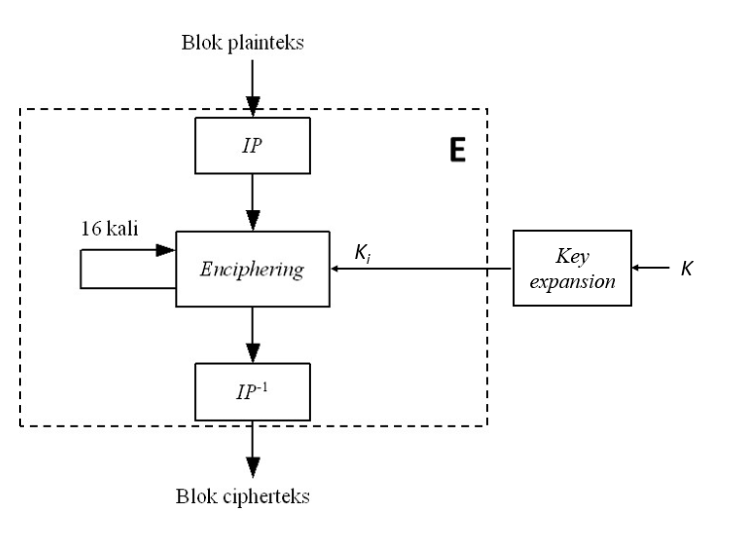
\includegraphics[width=0.85\linewidth, height=0.82\textheight, keepaspectratio]{figures/skema-enkripsi-des.png}
    \caption{Skema menyeluruh enkripsi DES: permutasi awal, 16 putaran dengan subkunci hasil pembangkitan kunci, dan inversi permutasi awal}
    \label{fig:skema-enkripsi-des}
    \sumber{Munir, \textit{IF4020 Kriptografi}, ITB.}
\end{figure}

\begin{figure}[htbp]
    \centering
    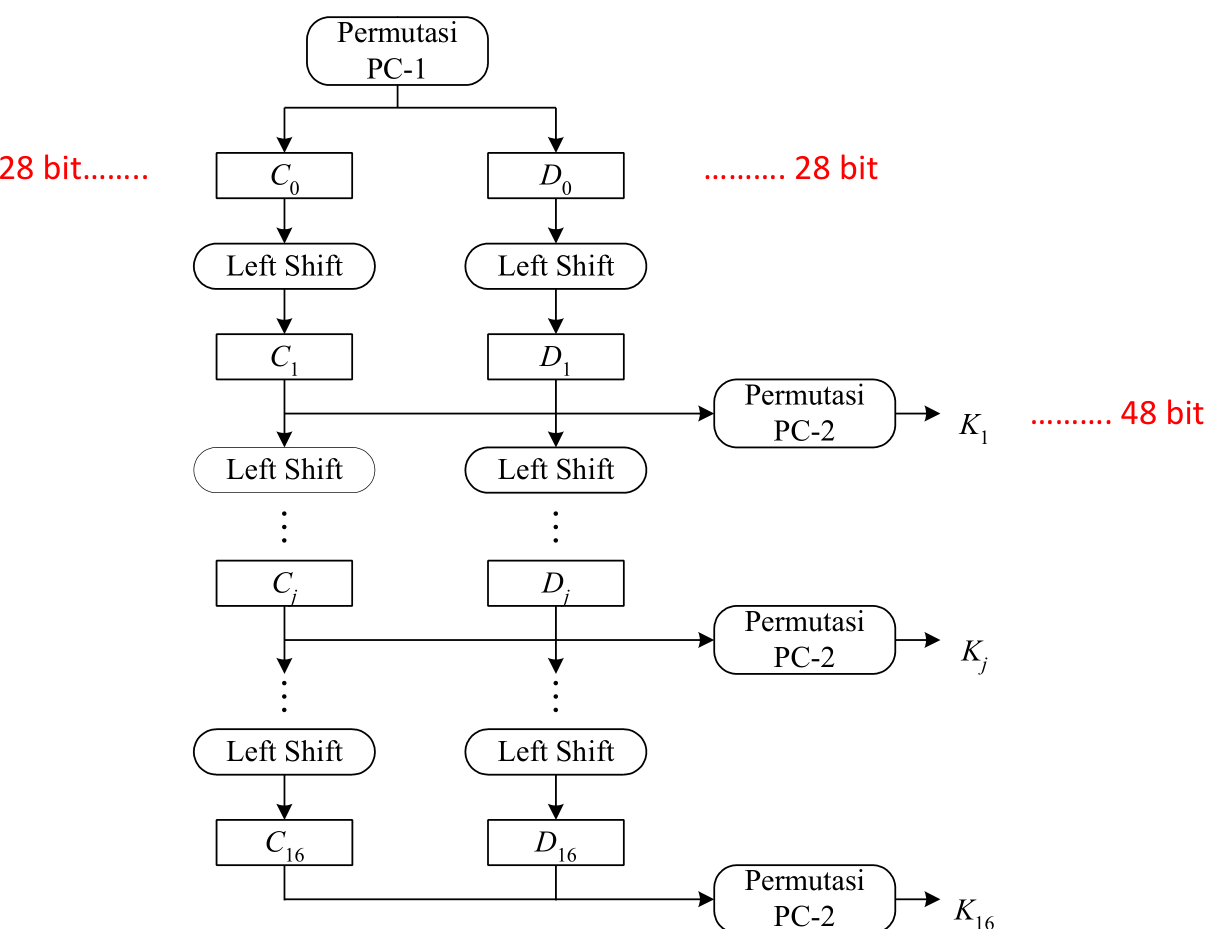
\includegraphics[width=0.9\linewidth, height=0.82\textheight, keepaspectratio]{figures/pembangkitan-kunci-des.png}
    \caption{Pembangkitan kunci internal DES: permutasi PC-1 membagi kunci 64 bit menjadi dua register 28 bit, lalu pergeseran dan permutasi PC-2 menghasilkan subkunci $K_1$ sampai $K_{16}$}
    \label{fig:pembangkitan-kunci-des}
    \sumber{Munir, \textit{IF4020 Kriptografi}, ITB.}
\end{figure}
